\subsection{Value functions in belief wealth space}\label{ssec:val-func}

First, we look at value functions found by using different utility functions in~\autoref{fig:val-func}.
As described in~\autoref{sec:methods} augmented state space encodes the wealth and the belief of the agent. 
Additionally, in our case, time can be derived from wealth exactly by $\text{time} = \frac{\text{wealth}}{\text{observation\ cost}}$.

In the first row, value functions found by the risk-neutral utility (identity function) and an exponential utility show that the induced behaviour is independent of time and risk is only modeled by the belief threshold the agent decides to sell at.
% TODO do we need a policy plot to make this clear?
Exponential utility sets this threshold with the $\lambda$ parameter, which is displayed above the plot.
Positive $\lambda$ models risk-seeking behavior, which results in selling with less belief.

In the second row, we see that the sinh utility function is able to model time dependent behaviour, e.g. selling at a fixed time step. We have parametrized sinh by the scaling and shifting of its input:

\begin{align*}
    U_\text{sinh}(v) := e^{v_1} - e^{-v_2} \text{, where\ } v_i = \text{scale_i}\cdot(v+\text{shift_i})
\end{align*}

First plot shows what we call a fixed time policy, where the agent sells at a specific wealth value.
Second plot shows 

Lastly, we present the dynamic utility function where $\lambda_i$ is selected from a logarithmically spaced sequence. The sequence range is displayed above each plot.

% TODO: use sinh with better parametrization

\begin{figure}[h]
    \centering
    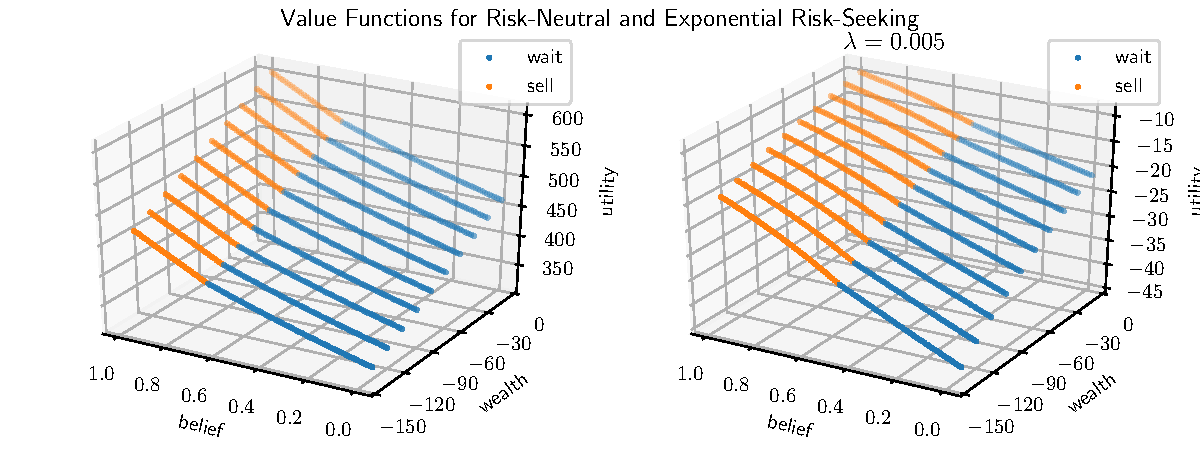
\includegraphics[width=0.99\linewidth]{img/exp_policy.pdf}\\
    \vspace{1cm}
    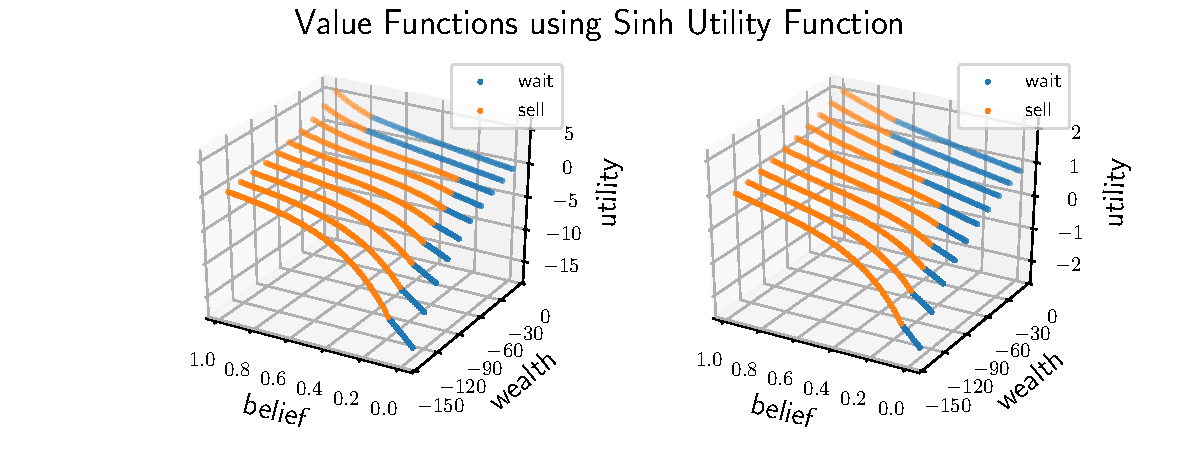
\includegraphics[width=0.99\linewidth]{img/sinh_policy.pdf}\\
    \vspace{1cm}
    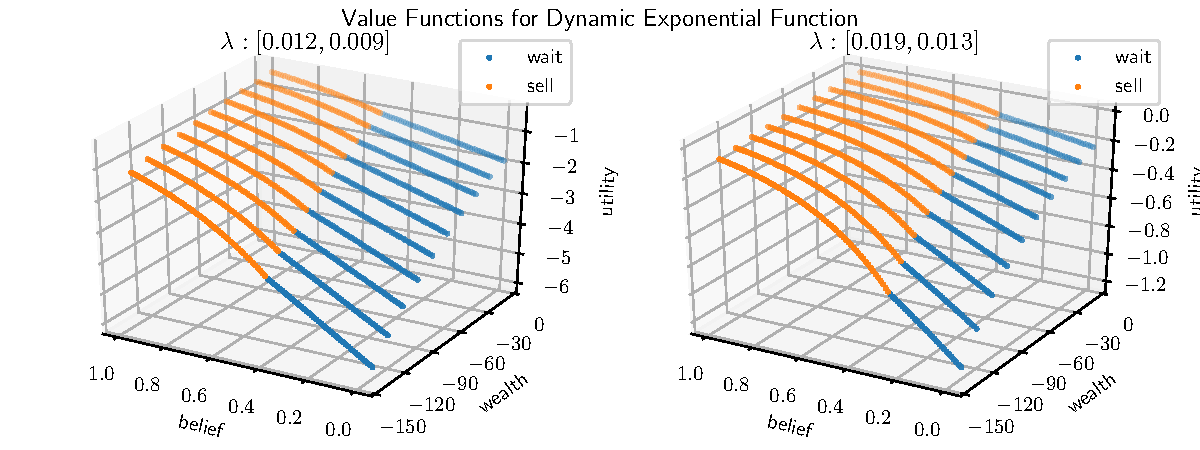
\includegraphics[width=0.99\linewidth]{img/dyn_policy.pdf}
    \caption{Value functions exhibiting different risk-behaviors; from top left: risk neutral agent (utility function is the identity function), risk-seeking agent with exponential utility function, two fixed time agents with different time thresholds, two agents with dynamic exponential utility function.}\label{fig:val-func}
\end{figure}

\subsection{From human behavior to utility functions}\label{ssec:human-behavior}

In~\autoref{ssec:val-func}, we have presented how different utility functions result in different policies.
However, our main goal is to derive a utility function and the corresponding risk parameters from behavioral data.
In literature, this is called \keyword{inverse reinforcement learning} \cite{TODO}.

Inverse reinforcement learning is challenging, thus, we only try a naive approach, which can be summarized in three steps: 1) observe behaviour, 2) estimate policy, and 3) derive utility functions and risk parameters using a grid-search.
This approach is plotted in~\autoref{fig:svm_vs_value}, and explained in following. 
First, we get behavioral data for a subject from the expert-setting of the experiment.
For each time step (i.e. year) of each trial we have a data point with the action subject took, the belief shown to the user and the year. These are plotted in~\autoref{fig:svm_vs_value} with blue for wait action, and orange for sell action.

Second, we estimate the policy using a SVM \cite{TODO} with cross-validation. SVM tries to fit a decision boundary, which minimizes the wait actions above and sell actions below this boundary.


The last step is to perform a grid search over utility functions and their parameters.
Each utility function and its parameters results in a value function from which a policy can be derived.
The goal of the grid search is to find the closest policy that is closest to the SVM decision boundary.

\begin{figure}[h]
    \centering
    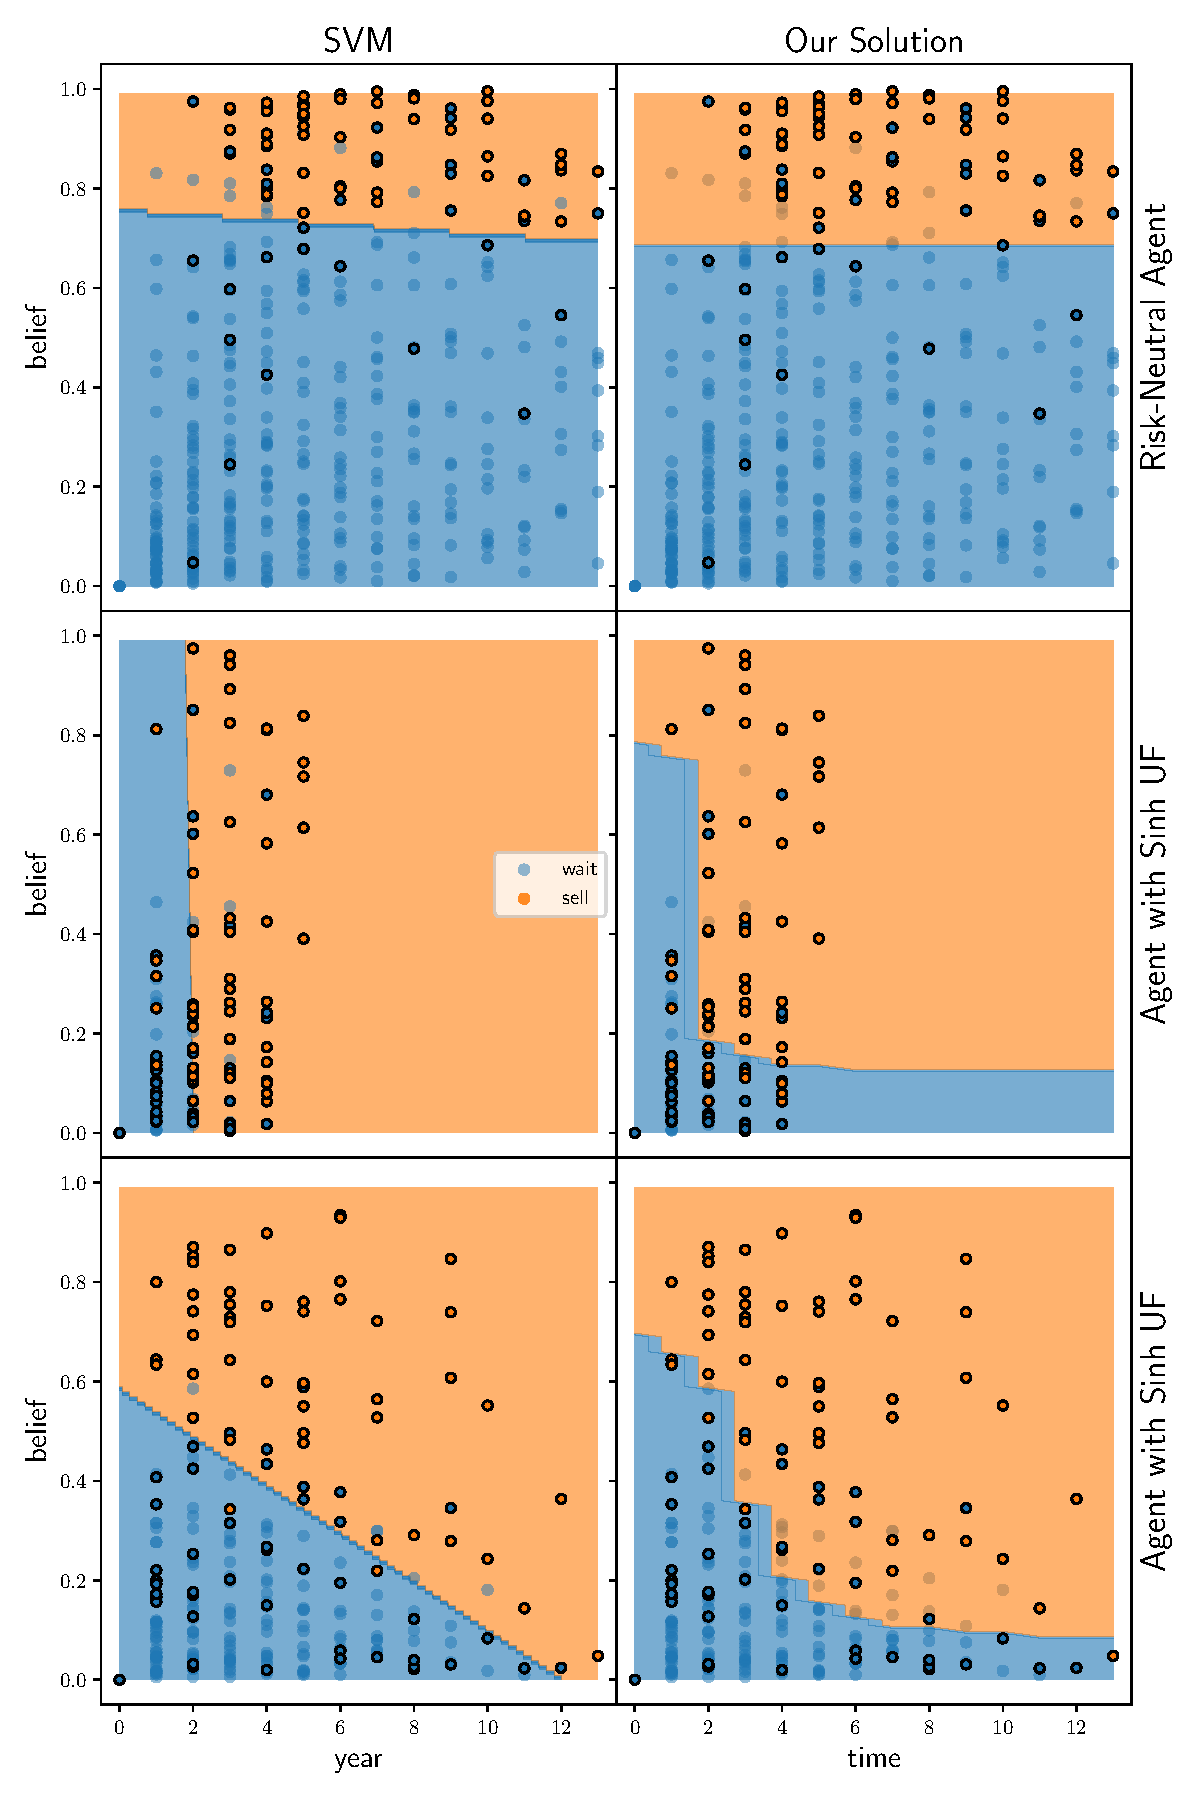
\includegraphics[width=0.99\linewidth]{img/fit}
    \caption{Examples from three human behaviors distinctly observed, and reproduced with RL agents. Behaviours by row: 1) Constant belief threshold, modelled by exponential utility, 2) Fixed time threshold, modelled by sinh utility, 3) Mixed strategy, modelled by dynamic exponential utility. Left column shows empirical optimal split of data using cross validation and linear kernel support vector machines, right column shows optimal policy found via grid-search.}
    \label{fig:svm_vs_value}
\end{figure}

\subsection{Analysis of agents}
After reproducing the human behavior with agents we can compare their performance, which is presented in~\autoref{fig:perf}.
First plot shows the average accumulated reward of each agent, and the second plot shows the ratio of sells in good state.
We observe couple of interesting things.

First, the risk-averse agent has a lower variance both on average reward, and ratio of selling in good state. However it has similar number of outliers in average reward to risk-neutral agent, which can be easily explained by the high selling threshold that results in long waiting time for the risk-averse agent.

Second, % TODO

\begin{figure}[h]
    \centering
    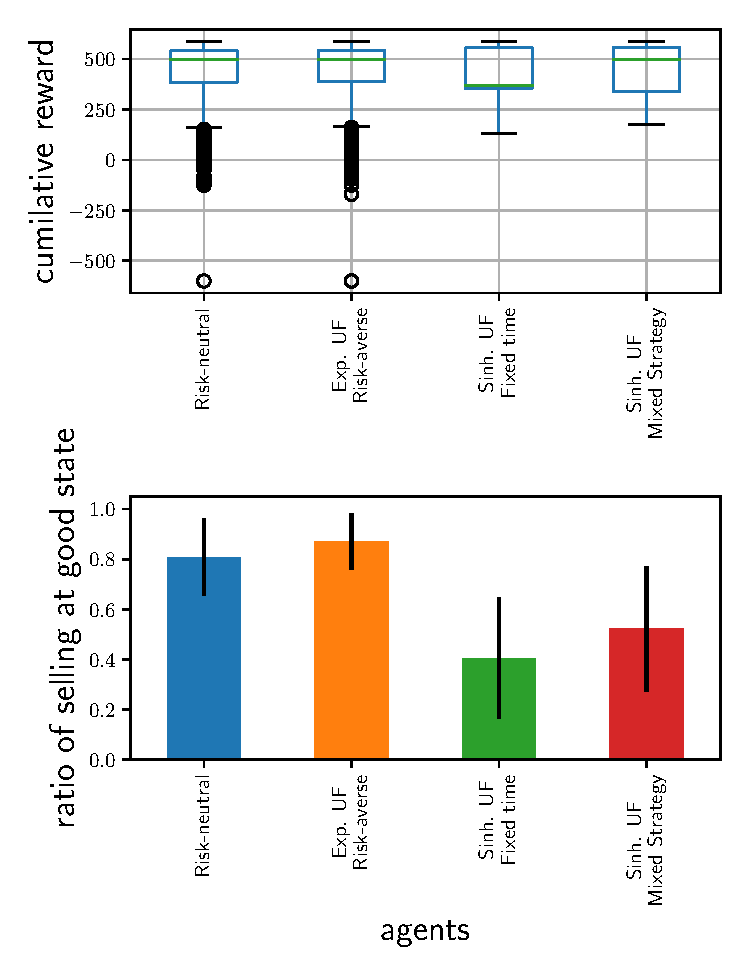
\includegraphics[width=0.99\linewidth]{img/performance.pdf}
    \caption{Average reward and ratio of selling in the good state.}\label{fig:perf}
\end{figure}
